\documentclass[conference]{IEEEtran}
\IEEEoverridecommandlockouts
% The preceding line is only needed to identify funding in the first footnote. If that is unneeded, please comment it out.
\usepackage{cite}
\usepackage{amsmath,amssymb,amsfonts}
\usepackage{algorithmic}
\usepackage{graphicx}
\usepackage{textcomp}
\usepackage{xcolor}
\usepackage{booktabs} % Include this in the preamble for better table lines
\usepackage{amsmath}
\usepackage{colortbl}
\usepackage{hyperref}
\usepackage[acronym]{glossaries}
\def\BibTeX{{\rm B\kern-.05em{\sc i\kern-.025em b}\kern-.08em
    T\kern-.1667em\lower.7ex\hbox{E}\kern-.125emX}}


\definecolor{htwg-teal}{cmyk}{1.0,0.0,0.5,0.0}

\newcommand{\MYhead}{\smash{\scriptsize
\hfil\parbox[t][\height][t]{\textwidth}{\centering
\begin{picture}(0,0) \put(-30,-30){\includegraphics[width=50mm]{htwg_in.png}} \end{picture} \hspace{4.8cm}
Team Project MSI - Winter Term 2023/24 and Summer Term 2024 \hspace{4cm} 18.08.2024\\
%Department of Computer Science\\
Professor: Prof. Dr. Oliver Dürr\\
\hspace{6cm}
%\textcolor{htwg-teal}{\underline{\hspace{ \textwidth}}}
\hfil\hbox{}}}}

\makeatletter
% normal pages
\def\ps@headings{%
\def\@oddhead{\MYhead}%
\def\@evenhead{\MYhead}}%
% title page
\def\ps@IEEEtitlepagestyle{%
\def\@oddhead{\MYhead}%
\def\@evenhead{\MYhead}}%
\makeatother

\begin{document}

\newacronym{knn}{KNN}{K-nearest-neigbours}


\title{Chatbot for the examination office
% {\footnotesize \textsuperscript{*}Note: Sub-titles are not captured in Xplore and
% should not be used}
% \thanks{Identify applicable funding agency here. If none, delete this.}
}

\author{
\IEEEauthorblockN{Benjamin Brünau}
\IEEEauthorblockA{
    \textit{HTWG Konstanz}\\
        Konstanz, Germany\\
        be391bru@htwg-konstanz.de
}
\and
\IEEEauthorblockN{Khadidja Kebaili}
\IEEEauthorblockA{
    \textit{HTWG Konstanz}\\
        Konstanz, Germany\\
        kh871keb@htwg-konstanz.de
}
\and
\IEEEauthorblockN{Joel Merath}
\IEEEauthorblockA{
    \textit{HTWG Konstanz}\\
        Konstanz, Germany\\
        joel.merath.fh@gmail.com
}
\and
\IEEEauthorblockN{Jan Schmidt}
\IEEEauthorblockA{
    \textit{HTWG Konstanz}\\
        Konstanz, Germany\\
        ja163sch@htwg-konstanz.de 
}
}


\maketitle

\begin{abstract} \\
The aim of this team project is to develop a chatbot adapted to the requirements of the examination office (Prüfungsamt) to automatically answer frequently asked questions based on provided documents (e.g. studies and examination regulations). Given the increasing demand for quick and accurate information access in academic institutions, this research focuses on designing and implementing a chatbot to streamline administrative processes. The performance and accuracy of the chatbot will be evaluated using various metrics, to measure its reliability and effectiveness.\\
These metrics will furthermore be used to measure how much of an improvement is achieved by finetuning a Large Language Model for this task and domain.
\end{abstract}


\section{Introduction}

In recent years, the use of artificial intelligence has gained significant attention in several areas. One of the emerging applications is the deployment of chatbots to handle routine inquiries, such as answering frequently asked questions of customers, employees, etc. \\
This paper focuses on developing a chatbot for the HTWG examination office that can automatically respond to frequently asked questions using existing documentation. Our aim is to improve the efficiency and accessibility of information for students and staff. The motivation behind this work lies in reducing the workload of administrative staff and providing timely, accurate information. Additionally, this research serves as a proof of concept, demonstrating the feasibility of implementing such a system in an academic administrative environment. The performance of the chatbot will be thoroughly evaluated using a variety of metrics to measure its effectiveness and reliability.

\section{Design and Implementation}

\subsection{Document retrieval}
Retrieving the correct document passage is crucial for ensuring accurate and relevant responses from the chatbot. Many search algorithms are using keywords as searching method. While these methods are effective for simple queries, they often fail to capture the contextual meaning, leading to suboptimal results.

To overcome these limitations, we used a semantic search method. This technique involves embedding both the queries and the documents into a high-dimensional space using a neural network, where semantically similar texts are represented by vectors in close proximity. To increase the chances of finding the correct information, multiple documents are retrieved. The count of how many documents are retrived is described with the \acrfull{knn} value. The retrieved documents are then passed to a Large Language Model (LLM) to generate the final response.

The document retrieval process requires several key steps. First, text extraction from various document formats such as PDF and DOCX is performed. We discovered that manual tuning of the extraction process—such as removing headers, footers, and combining the text into coherent passages—significantly improved the accuracy of the retrieval. The processed text is then divided into chunks using unique characters, ensuring that the passages are meaningfully segmented.

To optimize our retrieval system, we conducted extensive testing with various embedding models and configurations. The goal was to verify whether the model could correctly identify relevant sections within the text. This was assessed by defining unique keywords and ensuring all keywords were present within the retrieved passage. The performance of different models and settings was rigorously evaluated, and the results are detailed in the subsequent section \ref{subsec:results_retrieval}.

\iffalse
Another challenge was the extraction of data from tables within PDFs. Standard extraction techniques often resulted in errors, such as missing information or incorrect data due to formatting issues. After evaluating several tools, including Optical Character Recognition (OCR) and advanced language models like ChatGPT, we concluded that current methods are insufficiently reliable for extracting tabular data. Consequently, we excluded tables from our retrieval process, marking this as an area for future research.
\fi



\subsection{Evaluation}

%For the evaluation of our chatbot, we utilized a combination of custom %and established metrics to thoroughly assess its performance. For that %reason we developed three custom metrics: \\
%A. Key-Word Score, which measures the presence of essential keywords %in the chatbot’s responses, \\
%B. Correct-Page-Score, which evaluates whether the chatbot accurately %identifies the correct source document and \\
%C. ChatGpt-Score [using ChatGPT to further gauge the quality of the %responses]  \\
%Additionally, we used several metrics, which are commonly used, such %as BLEU Score, a metric that assesses the overlap of n-grams between %the generated response and a reference answer, and Rouge Score, which %evaluates the semantic accuracy of responses by comparing them to a %set of expected answers. Cosine-Similarity was also employed to %measure the similarity between the vectors of the generated and %reference texts. Finally, Prompt engineering played a crucial role in %fine-tuning the chatbot's interactions, ensuring that the inputs were %crafted to elicit the most accurate and relevant responses. The %results from all these metrics were visualized using Promptfoo, %providing a comprehensive overview of the chatbot's performance.

To evaluate the performance of the chatbot, a combination of custom and established metrics was employed. Three custom metrics were developed: the Keyword Score, which assesses the presence of essential keywords in the chatbot’s responses; the Correct-Page Score, which determines whether the chatbot accurately identifies the correct source document; and the ChatGPT Score, which utilizes ChatGPT to further evaluate the quality of the responses.

In addition to these custom metrics, several established metrics were used to analyze the chatbot’s performance on both semantic and textual levels. The semantic evaluation, which was given higher priority, is particularly critical for the chatbot’s application within an examination office, where precise and contextually relevant responses are required. The Keyword Score plays a central role in ensuring that key terms are present in the responses. Cosine Similarity was employed to measure the semantic alignment between the generated responses and the reference answers, thereby verifying the accuracy and relevance of the content.

For the analysis at the word and text level, which was weighted less heavily, Edit Distance, ROUGE-1, ROUGE-2, ROUGE-L, and Jaccard Similarity were utilized. Although these metrics were assigned a lower weight, their importance remains, as they assess the textual precision and consistency of the responses. These metrics ensure that the chatbot’s outputs are not only semantically correct but also well-formulated and closely aligned with the reference texts. This is particularly significant in formal contexts, such as within an examination office, where the structural integrity of responses is critical.

Furthermore, \href{https://www.promptfoo.dev/}{Promptfoo} was utilized to test the Retrieval-Augmented Generation (RAG) system with a diverse set of large language models (LLMs). A wide range of reference questions and answers were compared with the outputs generated by the LLMs, and the respective scores were calculated. This approach enabled the identification of LLMs that are most effective in conjunction with the RAG system and are likely to produce the most accurate responses. The average of the weighted metrics, including correctness, specificity, and relevance, serves as a key indicator in selecting the optimal model, providing a clear assessment of each model’s performance.

Prompt engineering played a crucial role in refining the chatbot’s interactions, ensuring that prompts were crafted to elicit the most accurate and relevant responses. The outcomes of these metrics were visualized using Promptfoo, providing a comprehensive overview of the chatbot’s performance.



\subsection{Finetuning}
Two primary approaches were taken for finetuning an LLM:

\begin{itemize}
\item Teaching the LLM the content of documents by finetuning it on specific paragraphs.
\item Enhancing the Retrieval Augmented Generation (RAG) process by training the model to extract relevant context and accurately answer questions based on it.
\end{itemize}

Given our computational constraints, we opted for parameter-efficient finetuning (PEFT) using LoRA (Low Rank Adaptation) instead of the more resource-intensive Full Fine Tuning. LoRA significantly reduces the number of parameters that need to be trained by approximating the weight update matrix with lower-rank matrices (as illustrated in Figure \ref{fig:LORA}). The training process was executed using Huggingface \href{https://huggingface.co/docs/transformers/de/index}{Transformers} and tracked via \href{https://wandb.ai/site}{wandb}. Datasets were synthetically created through API requests to \textit{ChatGPT4o}.
\newline
\newline




\begin{figure}[]
    \centering
    \includegraphics[width=\columnwidth]{lora.png}
    \caption{Weight update: Full Fine Tuning vs LoRA}
    \label{fig:LORA}
\end{figure}




\section{Results}
\subsection{Retrieval}
\label{subsec:results_retrieval}
The effectiveness of our document retrieval process was evaluated using several metrics, as detailed in Table \ref{tab:performance}. We tested multiple embedding models, including \href{https://huggingface.co/sentence-transformers/all-MiniLM-L6-v2}{all-MiniLM-L6-v2} (Model A), \href{https://huggingface.co/sentence-transformers/all-mpnet-base-v2}{all-mpnet-base-v2} (Model B), and \href{https://huggingface.co/sentence-transformers/paraphrase-multilingual-MiniLM-L12-v2}{paraphrase-multilingual-MiniLM-L12-v2} (Model C). The models were evaluated across different context sizes (1024, 2048, and 4096) and varying \acrshort{knn} settings (1, 3, 5, and 10). As demonstrated in Table \ref{tab:performance}, Models B and C exhibited the most optimal performance outcomes. Given that Model C yielded superior outcomes solely in consideration of the keywords, irrespective of the passage, in comparison to Model B, this model was selected for the subsequent tests. Furthermore, the chunk size of 2048 exhibited slightly enhanced performance metrics in comparison to 1024 or 4096.
The optimal chunk size for text segmentation was determined to be 2048 tokens, with a chunk overlap of 256 tokens. All processed text chunks were stored in a ChromaDB, an open-source vector database, thereby facilitating efficient retrieval during chatbot operation.



\begin{table}[h!]
\centering
\begin{tabular}{|l|c|c|c|c|}
\hline
\textbf{Model} & \textbf{Knn} & \textbf{Context size} & \textbf{Context size} & \textbf{Context size} \\ 
 &  & \textbf{1024} & \textbf{2048} & \textbf{4096} \\ \hline
A & 1 & 0.24 & 0.28 & 0.21 \\ \hline
B & 1 & 0.41 & 0.48 & 0.45 \\ \hline
\rowcolor{gray!30} C & 1 & 0.52 & 0.52 & 0.48 \\ \hline
\specialrule{1.5pt}{0pt}{0pt} % Thicker line after every 3 rows
A & 3 & 0.38 & 0.45 & 0.38 \\ \hline
\rowcolor{gray!30} B & 3 & 0.62 & 0.62 & 0.66 \\ \hline
C & 3 & 0.59 & 0.59 & 0.59 \\ \hline
\specialrule{1.5pt}{0pt}{0pt} % Thicker line after every 3 rows
A & 5 & 0.62 & 0.72 & 0.66 \\ \hline
\rowcolor{gray!30} B & 5 & 0.72 & 0.72 & 0.72 \\ \hline
C & 5 & 0.69 & 0.72 & 0.72 \\ \hline
\specialrule{1.5pt}{0pt}{0pt} % Thicker line after every 3 rows
\rowcolor{gray!30} A & 10 & 0.90 & 0.86 & 0.86 \\ \hline
B & 10 & 0.79 & 0.79 & 0.79 \\ \hline
\rowcolor{gray!30} C & 10 & 0.86 & 0.90 & 0.86 \\ \hline
\end{tabular}
\caption{Accuracy of models with different context sizes and K-nearest neighbors (Knn) finding the correct context passage. The best model (highest average of scores) in each Knn group is highlighted with a gray background.}
\label{tab:performance}
\begin{tablenotes}
\small
\item A = \href{https://huggingface.co/sentence-transformers/all-MiniLM-L6-v2}{all-MiniLM-L6-v2}, B = \href{https://huggingface.co/sentence-transformers/all-mpnet-base-v2}{all-mpnet-base-v2}, C = \href{https://huggingface.co/sentence-transformers/paraphrase-multilingual-MiniLM-L12-v2}{paraphrase-multilingual-MiniLM-L12-v2}
\end{tablenotes}
\end{table}



\begin{table}[h!]
\centering
\begin{tabular}{|l|c|c|c|c|}
\hline
\textbf{Model} & \textbf{Knn} & \textbf{Context size} & \textbf{Context size} & \textbf{Context size} \\ 
 &  & \textbf{1024} & \textbf{2048} & \textbf{4096} \\ \hline
                    A & 1 & 0.32 & 0.34 & 0.28 \\ \hline
                    B & 1 & 0.45 & 0.55 & 0.52 \\ \hline
\rowcolor{gray!30}  C & 1 & 0.56 & 0.56 & 0.51 \\ \hline
\specialrule{1.5pt}{0pt}{0pt} % Thicker line after every 3 rows
                    A & 3 & 0.55 & 0.65 & 0.70 \\ \hline
\rowcolor{gray!30}  B & 3 & 0.72 & 0.78 & 0.72 \\ \hline
                    C & 3 & 0.75 & 0.75 & 0.70 \\ \hline
\specialrule{1.5pt}{0pt}{0pt} % Thicker line after every 3 rows
                    A & 5 & 0.69 & 0.78 & 0.73 \\ \hline
                    B & 5 & 0.78 & 0.78 & 0.79 \\ \hline
\rowcolor{gray!30}  C & 5 & 0.78 & 0.80 & 0.85 \\ \hline
\specialrule{1.5pt}{0pt}{0pt} % Thicker line after every 3 rows
                    A & 10 & 0.95 & 0.91 & 0.88 \\ \hline
                    B & 10 & 0.84 & 0.84 & 0.85 \\ \hline
\rowcolor{gray!30}  C & 10 & 0.94 & 0.95 & 0.91 \\ \hline
\end{tabular}
\caption{Accuracy of models with different context sizes and K-nearest neighbors (Knn) finding passages with korrect keywords. The best model (highest average of scores) in each Knn group is highlighted with a gray background.}
\label{tab:performance_keywords}
\begin{tablenotes}
\small
\item A = \href{https://huggingface.co/sentence-transformers/all-MiniLM-L6-v2}{all-MiniLM-L6-v2}, B = \href{https://huggingface.co/sentence-transformers/all-mpnet-base-v2}{all-mpnet-base-v2}, C = \href{https://huggingface.co/sentence-transformers/paraphrase-multilingual-MiniLM-L12-v2}{paraphrase-multilingual-MiniLM-L12-v2}
\end{tablenotes}
\end{table}

\newpage
\subsection{Finetuning}

Finetuning an LLM via PEFT on document paragraphs with the goal of teaching it new knowledge and expecting accurate question answering does not yield satisfying results in practice. Although the LLM may learn to mimic the style of the documents, it tends to hallucinate frequently, producing names and details that are no more likely to be correct than incorrect.

In contrast, instruction finetuning aimed at improving the model's performance in Retrieval Augmented Generation leads to significant performance gains when answering questions based on a given context. This improvement can be further enhanced by training the LLM on a dataset where answers are structured as Chain of Thought (COT) responses, guiding the model to work through problems step by step. The dataset used for finetuning with COT answers was approximately twice the size, which may have also contributed to the improved performance (192 vs. 452 rows). The model's enhanced ability to extract relevant excerpts, identify key elements, and formulate answers is evident in Figure \ref{fig:FINETUNE_OVER_TIME}}, where finetuned models trained on COT answers outperformed others.

Interestingly, models trained on noisy, synthetic datasets that were not manually cleaned or validated before finetuning performed slightly better in some metrics, such as Keyword Score. For example, \texttt{mistral-rag-instruct.HF-NEW} (finetuned on a cleaned dataset) and \texttt{mistral-rag-instruct.HF-OLD} (finetuned on a noisy dataset) in Figure \ref{fig:FINETUNE_OVER_TIME} show that the latter had a slight edge, though this could be attributed to various factors such as dataset size or random variation.

The semantic correctness of the generated responses was nearly on par with proprietary models like \texttt{GPT-3.5-turbo} and the finetuned models even outperformed it in keyword extraction. However, they scored lower in metrics comparing text similarity, since they generate more verbose responses through their Chain of Thought answer process, leading to greater divergence from the reference answers. This is reflected in Figure \ref{fig:FINETUNE_OVER_TIME} (note that while cosine similarity is normalized to 1.0, the actual cosine similarity values can be seen in Figure \ref{fig:FINETUNE_ALL_METRICS}).

\section{Conclusion and Recommendation}

Our findings suggest that developing a chatbot for the examination office is feasible, especially given the rapid advancements in this technology. However, there remains a significant level of uncertainty due to the tendency of large language models (LLMs) to generate incorrect or fabricated information when they lack sufficient knowledge. This issue persists even in advanced LLMs like ChatGPT, despite the substantial financial investments made in their development, making it likely that our local model will struggle to match their performance. Given the importance of accurate information in the context of an examination office, we recommend using the chatbot with caution, ensuring that it always provides references to the source documents and specific page numbers. Additionally, further exploration of options such as integrating multiple LLMs or other advanced techniques should be pursued to enhance the reliability of the system.

%\section*{Acknowledgment}

%\section*{References}

\newpage

%\section{Figures}




\begin{figure*}[]
    \centering
    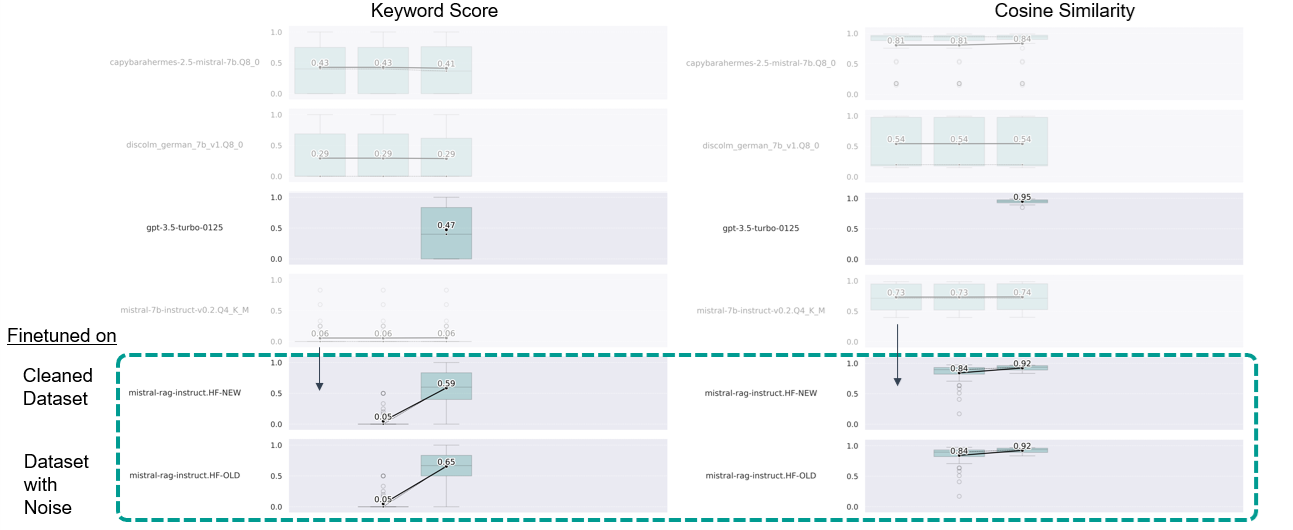
\includegraphics[width=\linewidth]{finetune-results-over-time.png}
    \caption{Finetuning - Semantic Performance over several evaluation runs}
    \label{fig:FINETUNE_OVER_TIME}
\end{figure*}

\begin{figure*}[]
    \centering
    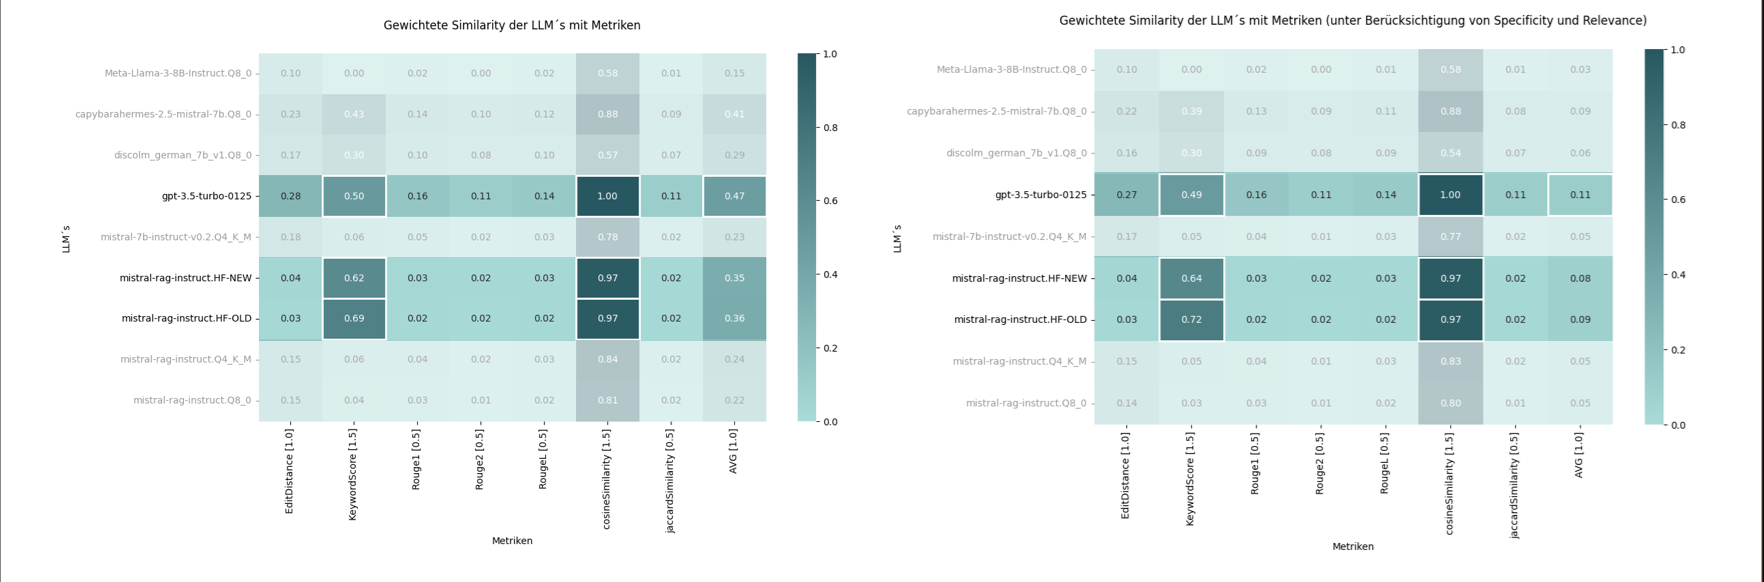
\includegraphics[width=\linewidth]{finetune-results-all-metrics.png}
    \caption{Finetuning - Comparison for all metrics on one evaluation run}
    \label{fig:FINETUNE_ALL_METRICS}
\end{figure*}






%\begin{thebibliography}{00}
%\end{thebibliography}
\vspace{12pt}

\end{document}

#if 0

\section{Strategy}
Before you begin to format your paper, first write and save the content as a 
separate text file. Complete all content and organizational editing before 
formatting. Please note sections \ref{AA}--\ref{SCM} below for more information on 
proofreading, spelling and grammar.

Keep your text and graphic files separate until after the text has been 
formatted and styled. Do not number text heads---{\LaTeX} will do that 
for you.

\subsection{Abbreviations and Acronyms}\label{AA}
Define abbreviations and acronyms the first time they are used in the text, 
even after they have been defined in the abstract. Abbreviations such as 
IEEE, SI, MKS, CGS, ac, dc, and rms do not have to be defined. Do not use 
abbreviations in the title or heads unless they are unavoidable.

\subsection{Units}
\begin{itemize}
\item Use either SI (MKS) or CGS as primary units. (SI units are encouraged.) English units may be used as secondary units (in parentheses). An exception would be the use of English units as identifiers in trade, such as ``3.5-inch disk drive''.
\item Avoid combining SI and CGS units, such as current in amperes and magnetic field in oersteds. This often leads to confusion because equations do not balance dimensionally. If you must use mixed units, clearly state the units for each quantity that you use in an equation.
\item Do not mix complete spellings and abbreviations of units: ``Wb/m\textsuperscript{2}'' or ``webers per square meter'', not ``webers/m\textsuperscript{2}''. Spell out units when they appear in text: ``. . . a few henries'', not ``. . . a few H''.
\item Use a zero before decimal points: ``0.25'', not ``.25''. Use ``cm\textsuperscript{3}'', not ``cc''.)
\end{itemize}

\subsection{Equations}
Number equations consecutively. To make your 
equations more compact, you may use the solidus (~/~), the exp function, or 
appropriate exponents. Italicize Roman symbols for quantities and variables, 
but not Greek symbols. Use a long dash rather than a hyphen for a minus 
sign. Punctuate equations with commas or periods when they are part of a 
sentence, as in:
\begin{equation}
a+b=\gamma\label{eq}
\end{equation}

Be sure that the 
symbols in your equation have been defined before or immediately following 
the equation. Use ``\eqref{eq}'', not ``Eq.~\eqref{eq}'' or ``equation \eqref{eq}'', except at 
the beginning of a sentence: ``Equation \eqref{eq} is . . .''

\subsection{\LaTeX-Specific Advice}

Please use ``soft'' (e.g., \verb|\eqref{Eq}|) cross references instead
of ``hard'' references (e.g., \verb|(1)|). That will make it possible
to combine sections, add equations, or change the order of figures or
citations without having to go through the file line by line.

Please don't use the \verb|{eqnarray}| equation environment. Use
\verb|{align}| or \verb|{IEEEeqnarray}| instead. The \verb|{eqnarray}|
environment leaves unsightly spaces around relation symbols.

Please note that the \verb|{subequations}| environment in {\LaTeX}
will increment the main equation counter even when there are no
equation numbers displayed. If you forget that, you might write an
article in which the equation numbers skip from (17) to (20), causing
the copy editors to wonder if you've discovered a new method of
counting.

{\BibTeX} does not work by magic. It doesn't get the bibliographic
data from thin air but from .bib files. If you use {\BibTeX} to produce a
bibliography you must send the .bib files. 

{\LaTeX} can't read your mind. If you assign the same label to a
subsubsection and a table, you might find that Table I has been cross
referenced as Table IV-B3. 

{\LaTeX} does not have precognitive abilities. If you put a
\verb|\label| command before the command that updates the counter it's
supposed to be using, the label will pick up the last counter to be
cross referenced instead. In particular, a \verb|\label| command
should not go before the caption of a figure or a table.

Do not use \verb|\nonumber| inside the \verb|{array}| environment. It
will not stop equation numbers inside \verb|{array}| (there won't be
any anyway) and it might stop a wanted equation number in the
surrounding equation.

\subsection{Some Common Mistakes}\label{SCM}
\begin{itemize}
\item The word ``data'' is plural, not singular.
\item The subscript for the permeability of vacuum $\mu_{0}$, and other common scientific constants, is zero with subscript formatting, not a lowercase letter ``o''.
\item In American English, commas, semicolons, periods, question and exclamation marks are located within quotation marks only when a complete thought or name is cited, such as a title or full quotation. When quotation marks are used, instead of a bold or italic typeface, to highlight a word or phrase, punctuation should appear outside of the quotation marks. A parenthetical phrase or statement at the end of a sentence is punctuated outside of the closing parenthesis (like this). (A parenthetical sentence is punctuated within the parentheses.)
\item A graph within a graph is an ``inset'', not an ``insert''. The word alternatively is preferred to the word ``alternately'' (unless you really mean something that alternates).
\item Do not use the word ``essentially'' to mean ``approximately'' or ``effectively''.
\item In your paper title, if the words ``that uses'' can accurately replace the word ``using'', capitalize the ``u''; if not, keep using lower-cased.
\item Be aware of the different meanings of the homophones ``affect'' and ``effect'', ``complement'' and ``compliment'', ``discreet'' and ``discrete'', ``principal'' and ``principle''.
\item Do not confuse ``imply'' and ``infer''.
\item The prefix ``non'' is not a word; it should be joined to the word it modifies, usually without a hyphen.
\item There is no period after the ``et'' in the Latin abbreviation ``et al.''.
\item The abbreviation ``i.e.'' means ``that is'', and the abbreviation ``e.g.'' means ``for example''.
\end{itemize}
An excellent style manual for science writers is \cite{b7}.

\subsection{Authors and Affiliations}
\textbf{The class file is designed for, but not limited to, six authors.} A 
minimum of one author is required for all conference articles. Author names 
should be listed starting from left to right and then moving down to the 
next line. This is the author sequence that will be used in future citations 
and by indexing services. Names should not be listed in columns nor group by 
affiliation. Please keep your affiliations as succinct as possible (for 
example, do not differentiate among departments of the same organization).

\subsection{Identify the Headings}
Headings, or heads, are organizational devices that guide the reader through 
your paper. There are two types: component heads and text heads.

Component heads identify the different components of your paper and are not 
topically subordinate to each other. Examples include Acknowledgments and 
References and, for these, the correct style to use is ``Heading 5''. Use 
``figure caption'' for your Figure captions, and ``table head'' for your 
table title. Run-in heads, such as ``Abstract'', will require you to apply a 
style (in this case, italic) in addition to the style provided by the drop 
down menu to differentiate the head from the text.

Text heads organize the topics on a relational, hierarchical basis. For 
example, the paper title is the primary text head because all subsequent 
material relates and elaborates on this one topic. If there are two or more 
sub-topics, the next level head (uppercase Roman numerals) should be used 
and, conversely, if there are not at least two sub-topics, then no subheads 
should be introduced.

\subsection{Figures and Tables}
\paragraph{Positioning Figures and Tables} Place figures and tables at the top and 
bottom of columns. Avoid placing them in the middle of columns. Large 
figures and tables may span across both columns. Figure captions should be 
below the figures; table heads should appear above the tables. Insert 
figures and tables after they are cited in the text. Use the abbreviation 
``Fig.~\ref{fig}'', even at the beginning of a sentence.

\begin{table}[htbp]
\caption{Table Type Styles}
\begin{center}
\begin{tabular}{|c|c|c|c|}
\hline
\textbf{Table}&\multicolumn{3}{|c|}{\textbf{Table Column Head}} \\
\cline{2-4} 
\textbf{Head} & \textbf{\textit{Table column subhead}}& \textbf{\textit{Subhead}}& \textbf{\textit{Subhead}} \\
\hline
copy& More table copy$^{\mathrm{a}}$& &  \\
\hline
\multicolumn{4}{l}{$^{\mathrm{a}}$Sample of a Table footnote.}
\end{tabular}
\label{tab1}
\end{center}
\end{table}

\begin{figure}[htbp]
\centerline{\includegraphics{fig1.png}}
\caption{Example of a figure caption.}
\label{fig}
\end{figure}

Figure Labels: Use 8 point Times New Roman for Figure labels. Use words 
rather than symbols or abbreviations when writing Figure axis labels to 
avoid confusing the reader. As an example, write the quantity 
``Magnetization'', or ``Magnetization, M'', not just ``M''. If including 
units in the label, present them within parentheses. Do not label axes only 
with units. In the example, write ``Magnetization (A/m)'' or ``Magnetization 
\{A[m(1)]\}'', not just ``A/m''. Do not label axes with a ratio of 
quantities and units. For example, write ``Temperature (K)'', not 
``Temperature/K''.
# endif
